%%%%%%%%%%%%%%%%%%%%%%%%%%%%%%%%%%%%%%%%%%%%%%%%%%%%%%%%%%%%%%%%%%%%%%
% COMP 1805
% December 9 2011
% Review questions
% Solutions by Alexis Beingessner, Michiel Smid
% Problems mostly taken from Rosen 6th, typed up by Simon Pratt
%%%%%%%%%%%%%%%%%%%%%%%%%%%%%%%%%%%%%%%%%%%%%%%%%%%%%%%%%%%%%%%%%%%%%%
\documentclass{article}

\usepackage{fullpage}
\usepackage{parskip}
\usepackage{enumitem}
\usepackage{amssymb}
\usepackage{graphicx}
\usepackage[usenames,dvipsnames]{color}

\newenvironment{proof}
{\color{PineGreen}\begin{list}{}%
         {\setlength{\leftmargin}{1cm}}%
         \item[]%
        \textbf{Proof:}
        
        }
{ $\square$\end{list}}

\newenvironment{answer}
{\color{PineGreen}\begin{list}{}%
         {\setlength{\leftmargin}{1cm}}%
         \item[]%
        \textbf{Answer: }}
{\end{list}}

\begin{document}

{\Huge COMP 1805 Review Questions}

From Rosen (6th ed.)

1.1: 33e) Construct a truth table for:

\[
(p \leftrightarrow q) \vee (\neg q \leftrightarrow r)
\]

\begin{answer}
\[\begin{array}{|c|c|c|c|c|c|}
\hline
p&q&r&p \leftrightarrow q&\neg q \leftrightarrow r&(p \leftrightarrow q) \vee (\neg q \leftrightarrow r)\\
\hline
T&T&T&T&F&T\\
T&T&F&T&T&T\\
T&F&T&F&T&T\\
T&F&F&F&F&F\\
F&T&T&F&F&F\\
F&T&F&F&T&T\\
F&F&T&T&T&T\\
F&F&F&T&F&T\\
\hline
\end{array}\]
\end{answer}
1.2: 30) Show that the following is a tautology:

\[
(p \vee q) \wedge (\neg p \vee r) \rightarrow (q \vee r)
\]

\begin{proof} 
\[\begin{array}{rcl}
&& (p \vee q) \wedge (\neg p \vee r) \rightarrow (q \vee r) \\
&\equiv& \neg((p \vee q) \wedge (\neg p \vee r)) \vee (q \vee r) \\
&\equiv& \neg(p \vee q) \vee \neg(\neg p \vee r) \vee (q \vee r) \\
&\equiv& (\neg p \wedge \neg q) \vee ( p \wedge \neg r) \vee (q \vee r) \\
&\equiv& (\neg p \wedge \neg q) \vee ( p \wedge \neg r) \vee q \vee r \\
&\equiv& ((\neg p \wedge \neg q) \vee q) \vee (( p \wedge \neg r) \vee r) \\
&\equiv& ((\neg p \vee q) \wedge (\neg q \vee q)) \vee ((p \vee r) \wedge (\neg r \vee r)) \\
&\equiv& ((\neg p \vee q) \wedge T) \vee ((p \vee r) \wedge T) \\
&\equiv& (\neg p \vee q) \vee (p \vee r) \\
&\equiv& \neg p \vee q \vee p \vee r \\
&\equiv& (\neg p \vee p) \vee q \vee r \\
&\equiv& T \vee q \vee r \\
&\equiv& T \\
\end{array}\]
\end{proof}

1.4: 33) Rewrite each of these statements so that negations appear only within predicates:

\begin{enumerate}[label=\alph{enumi})]
\item $ \neg \forall x \forall y P(x,y) $
\begin{answer}$ \exists x \exists y \neg P(x,y) $\end{answer}
\item $ \neg \forall y \exists x P(x,y) $
\begin{answer}$ \exists y \forall x \neg P(x,y) $\end{answer}
\item $ \neg \forall y \forall x (P(x,y) \vee Q(x,y)) $
\begin{answer}$ \exists y \exists x (\neg P(x,y) \wedge \neg Q(x,y)) $\end{answer}
\item $ \neg ( \exists x \exists y \neg P(x,y) \wedge \forall x \forall y Q(x,y)) $
\begin{answer}$ ( \forall x \forall y P(x,y) \vee \exists x \exists y \neg Q(x,y)) $\end{answer}
\item $ \neg \forall x ( \exists y \forall z P(x,y,z) \wedge \exists z \forall y P(x,y,z)) $
\begin{answer}$  \exists x ( \forall y \exists z \neg P(x,y,z) \vee \forall z \exists y \neg P(x,y,z)) $\end{answer}
\end{enumerate}

1.6: 39) Prove that at least one of the real numbers $a_1,a_2,...,a_n$ is greater than or equal to the average of these numbers.

\begin{proof}
Assume this is not the case. That is, that $a_1,a_2,...,a_n<(a_1+a_2+...+a_n)/n$. Then, $a_1+a_2+...+a_n<n(a_1+a_2+...+a_n)/n=a_1+a_2+...+a_n$, which is a contradiction. Therefore at least one of $a_1,a_2,...,a_n$ must be greater than or equal to their average.
\end{proof}

1.6: 40) Use Exercise 39 to show that if the first 10 positive integers are placed around a circle, in any order, there exist three integers in consecutive locations around the circle that have a sum greater than or equal to 17.
\begin{proof}
If we were to add the sum of every triplet of adjacent numbers, we would get a number 3 times as big as the original sum of the numbers 1-10, because every number would be counted three times. However there is the same number of triplets as there were original numbers. To see this, note that every triplet can be uniquely defined by which number was picked as the first. Therefore, the average of these triplet sums is three times as big as the average of 1-10. Since the average of 1-10 was 5.5, the average of these triplet sums is 16.5. As we have shown in exercise 39, at least one of these triplet sums must be greater than or equal to the average. Since we are adding integers, the sum must be an integer, so there must be a sum that is greater than or equal to 17.
\end{proof}
1.7: 32) Prove that $\sqrt[3]{2}$ is irrational.

\begin{proof}
Assume this is not the case. That is, $\sqrt[3]{2}$ is rational. Then we may write $\sqrt[3]{2}$ as $\frac{a}{b}$, where $a$ and $b$ are integers that share no common factor, and $b\neq 0$. Then:

\[\begin{array}{rcl}
\sqrt[3]{2} &=& \frac{a}{b}\\
2 &=& \frac{a^3}{b^3}\\
2b^3 &=& a^3\\
\end{array}\]

Since $a^3$ is even, $a$ must be even. Therefore we may express $a$ as $2k$, where $k$ is some integer. Then: 

\[\begin{array}{rcl}
2b^3 &=& a^3\\
2b^3 &=& (2k)^3\\
2b^3 &=& 8k^3\\
b^3 &=& 4k^3\\
\end{array}\]

Then $b^3$ and $b$ are also even. However this means both $a$ and $b$ have a common factor of $2$, which contradicts how we defined them. Our assumption is false, therefore $\sqrt[3]{2}$ is irrational.
\end{proof}

2.1: 19c) Find the power set of $ \{ \emptyset , \{ \emptyset \} \} $
\begin{answer} $\{\{ \emptyset , \{ \emptyset \} \}, \{ \emptyset \}, \{\{ \emptyset \}\}, \emptyset   \}$\end{answer}
2.4: 31) Determine whether each of these sets is countable or uncountable.  For those that are countable, exhibit a one-to-one correspondence between the set of natural numbers and that set.

\begin{enumerate}[label=\alph{enumi})]
\item the negative integers
\begin{proof} We may write the listing -1,-2,-3,... Therefore the negative integers are countable. \end{proof}
\item the even integers
\begin{proof} We may write the listing 0,2,-2,4,-4,... Therefore the even integers are countable. \end{proof}
\item the real numbers between 0 and $1/2$
\begin{proof} Assume that the real numbers from 0 to $1/2$ are countable. Then, we may order them $r_1,r_2,r_3,...$ and so on. Now define the number $r$ such that kth digit of its decimal expansion is 1 if $r_k's$ kth digit is 0, and 0 otherwise. First, note that $0>r>1/2$. Also note that this number differs from all $r_k$ at the $kth$ digit, so it is not included in this ordering. This contradicts that we had an ordering of all real numbers between 0 and $1/2$. Therefore our assumption is false, and this set is not countable. \end{proof}

\begin{proof} We already know that the real numbers from 0 to 1 are not countable. Further, we can construct a bijection from that set to the set of real numbers from 0 to 1/2 with the transformation $f(x) = x/2$. Therefore they are the same size, and this set is also not countable.\end{proof}
\item integers that are multiples of 7
\begin{proof} We may write the listing 0,7,-7,14,-14,... Therefore the multiples of 7 are countable. \end{proof}
\end{enumerate}

3.2: 24)

\begin{enumerate}[label=\alph{enumi})]
\item Show that $3x + 7$ is $\Theta (x)$
\begin{proof}
\[\begin{array}{rclr}
&&3x+7&\\
&\leq&3x+7x	&	x\geq 1\\
&=&10x & \\
\end{array}\]
Therefore $3x+7$ is $O(x)$, for $c=10$, $n=1$
\[\begin{array}{rclr}
&&3x+7&\\
&\geq&3x	&	x\geq 1\\
\end{array}\]
Therefore $3x+7$ is $\Omega(x)$, for $c=3$, $n=1$\\
Therefore $3x+7$ is $\Theta (x)$.
\end{proof}
\item Show that $2x^2+x-7$ is $\Theta (x^2)$
\begin{proof}
\[\begin{array}{rclr}
&&2x^2+x-7&\\
&\leq&2x^2+x^2	&	x\geq 1\\
&=&3x^2 & \\
\end{array}\]
Therefore $2x^2+x-7$ is $O(x^2)$, for $c=3$, $n=1$
\[\begin{array}{rclr}
&&2x^2+x-7&\\
&\geq&2x^2-7	&	\\
&\geq&x^2		& x^2 \geq 7 \\
&				& x \geq \sqrt{7} \\
\end{array}\]
Therefore $2x^2+x-7$ is $\Omega(x^2)$, for $c=1$, $n=\sqrt{7}$\\
Therefore $2x^2+x-7$ is $\Theta (x^2)$.
\end{proof}
\item Show that $\lfloor x + 1/2 \rfloor$ is $\Theta (x)$
\begin{proof}
\[\begin{array}{rclr}
&&\lfloor x + 1/2 \rfloor&\\
&\leq&x + 1/2	&		\\
&\leq&x + 1/2x	&	x \geq 1	\\
&=&3/2x			& \\
\end{array}\]
Therefore $\lfloor x + 1/2 \rfloor$ is $O(x)$, for $c=3/2$, $n=1$
\[\begin{array}{rclr}
&&\lfloor x + 1/2 \rfloor&\\
&\geq& x	&	x\geq 1\\
\end{array}\]
Therefore $\lfloor x + 1/2 \rfloor$ is $\Omega(x)$, for $c=1$, $n=1$\\
Therefore $\lfloor x + 1/2 \rfloor$ is $\Theta (x)$.
\end{proof}
\item Show that $log(x^2+1)$ is $\Theta (log_2(x))$
\begin{proof}
\[\begin{array}{rclr}
&&log(x^2+1)&\\
&=&log((x+1)(x-1))	&		\\
&\leq&log((x+1)(x+1))&	x \geq e	\\
&=&log((x+1)^2)&		\\
&=&2log(x+1)&		\\
&\leq&2log(x+x)&		\\
&=&2log(2x)&		\\
&=&2log(x) + log(2)&		\\
&=&2log(x) + log(2)log(x)&		\\
&=&2log(2)log(x)&		\\
&=&2log(2)log_2(x)/log_2(e)&		\\
\end{array}\]
Therefore $log(x^2+1)$ is $O(log_2(x))$, for $c=2log(2)/log_2(e)$, $n=e$
\[\begin{array}{rclr}
&&log(x^2+1)&\\
&\geq& log(x^2)	&	x\geq e\\
&=& 2log(x)	&	\\
&=& 2log_2(x)/log_2(e)	&	\\
\end{array}\]
Therefore $log(x^2+1)$ is $\Omega(log_2(x))$, for $c=2/log_2(e)$, $n=e$\\
Therefore $log(x^2+1)$ is $\Theta (log_2(x))$.
\end{proof}
\item Show that $log_{10}x$ is $\Theta (log_2(x))$
\begin{proof}
\[\begin{array}{rclr}
&&log_{10}x&\\
&=&log_{2}x/log_{2}10	&	x \geq 1	\\
\end{array}\]
Therefore $log_{10}x$ is $O(log_2(x))$ and $\Omega(log_2(x))$, for $c=log_{2}10$, $n=1$
Therefore $log_{10}x$ is $\Theta (log_2(x))$.
\end{proof}
\end{enumerate}

4.1: 21) Prove that $2^n > n^2$ if $n$ is an integer greater than 4

\begin{proof}
Base case (n=5):
$2^5 = 32 > 25 = 5^2$

Inductive hypothesis:
Assume $2^k > k^2$ for some $k \geq 5$.

Consider $k+1$:
\[\begin{array}{rclr}
&& 2^{k+1}& \\
&=& 2(2^k) & \\
&>& 2k^2 & \textrm{by inductive hypothesis} \\
&>& k^2 + 2k + 1 & \textrm{when }k^2>2k+1\textrm{, which is true when }k \geq 5 \\
&=& (k+1)^2 &\\
\end{array}\]

Therefore $2^n > n^2$ if $n$ is an integer greater than 4.\end{proof}

4.1: 31) Prove that 2 divides $n^2 + n$ whenever $n$ is a positive integer

\begin{proof} Assume $n$ is even, then $n = 2k$ for some integer $k$. Then 
\[\begin{array}{rcl}
&&n^2 + n \\
&=& (2k)^2 + 2k \\
&=& 4k^2 + 2k \\
&=& 2(k^2 + k)
\end{array}\]

Then $n^2 + n$ is divisible by 2. Assume $n$ is odd, then $n = 2k+1$ for some integer $k$. Then 
\[\begin{array}{rcl}
&&n^2 + n \\
&=& (2k+1)^2 + 2k+1\\
&=& 4k^2 +4k + 1 + 2k + 1 \\
&=& 2(2k^2 + 3k + 1)
\end{array}\]

Then $n^2 + n$ is divisible by 2. Therefore $n^2 + n$ is always divisible by 2.\end{proof}

\begin{proof}Note that $\Sigma^n_{k=1} k = (n^2+n)/2$. Clearly, as the sum of all positive integers, 
this sum must be a positive integer. So $n^2+n$ must always be divisible by 2, if n is positive.\end{proof}

\begin{proof}
$n^2 + n = n(n+1)$, the product of two consecutive integers; one of n and n+1 is even.
\end{proof}

4.3: 13) Where $f_n$ is the $n$th Fibonacci number, prove that

\[
f_1 + f_3 + ... + f_{2n-1} = f_{2n}
\]

\begin{proof}
Base case (n=1):
$f_1 = 1 = f_2$

Inductive hypothesis:
Assume $f_1 + f_3 + ... + f_{2k-1} = f_{2k}$ for some $k \geq 1$.

Consider $k+1$:
\[\begin{array}{rclr}
&& f_1 + f_3 + ... + f_{2k-1} + f_{2k+1}& \\
&=& f_{2k} + f_{2k+1} & \textrm{by inductive hypothesis} \\
&=& f_{2k+2} & \textrm{by definition of Fibonacci} \\
\end{array}\]

Therefore $f_1 + f_3 + ... + f_{2n-1} = f_{2n}$ for all $n \geq 1$.\end{proof}

5.1: 31) How many strings of eight English letters are there

\begin{enumerate}[label=\alph{enumi})]
\item that contain no vowels, if letters can be repeated?
\begin{answer}$ 21^8 $\end{answer}
\item that contain no vowels, if letters cannot be repeated?
\begin{answer}$ 21!/13! $\end{answer}
\item that start with a vowel, if letters can be repeated?
\begin{answer}$ 5(26^7) $\end{answer}
\item that start with a vowel, if letters cannot be repeated?
\begin{answer}$ 5(25!/18!) $\end{answer}
\item that contain at least one vowel, if letters can be repeated?
\begin{answer}$ 26^8 - 21^8 $\end{answer}
\item that contain exactly one vowel, if letters can be repeated?
\begin{answer}$ 5 {8 \choose 1} 21^7 $\end{answer}
\item that start with X and contain at least one vowel, if letters can be repeated?
\begin{answer}$ 26^7 - 21^7$\end{answer}
\item that start and end with X and contain at least one vowel, if
  letters can be repeated?
\begin{answer}$ 26^6 - 21^6$\end{answer}
\end{enumerate}

5.2: 9(modified) what is the minimum number of students, each of whom
comes from one of the 13 provinces and territories, who must be
enrolled in a university to guarantee that there are at least 100 who
come from the same province or territory?

\begin{answer}We know that if we have $n$ elements in $k$ containers that there exists a container with at least $\lceil n/k \rceil$ elements. If we know $k=13$ and want the smallest $n$ such that $\lceil n/k \rceil = 100$, we must pick the smallest $n$ such that $n/k>99$. Then we may solve $n/13 = 99$ for $n=1287$. Adding one to this gives us our final solution of $n=1288$. \end{answer}

5.2: 15) How many numbers must be selected from the set
$\{1,2,3,4,5,6\}$ to guarantee that at least one pair of these numbers
add up to 7?

\begin{answer}The only pairs that add to 7 are 1+6, 2+5, and 3+4. Therefore if we ever have two of the elements from any of these pairs, we will have such a pair. In the worst case we will first pick one from each pair, and then we are guaranteed to get a full pair on the fourth try. Therefore we must take at least 4 numbers to guarantee a sum to 7.\end{answer}

5.3: 38) How many ways are there to select 12 countries in the United
Nations to serve on a council if 3 are selected from a block of 45, 4
are selected from a block of 57, and the others are selected from the
remaining 69 countries?

\begin{answer}${45 \choose 3}{57 \choose 4}{69 \choose 5}$\end{answer}

5.4: 9) What is the coefficient of $x^{101}y^{99}$ in the expansion of
$(2x-3y)^{200}$?

\begin{answer}$-{200 \choose 101}2^{101} 3^{99}$\end{answer}

5.5: 11) How many ways are there to choose eight coins from a piggy
bank containing 100 identical pennies and 80 identical nickels?
\begin{answer}If we take n pennies, the remaining 8-n coins must be nickels. Since we have 9 choices of n, there are 9 ways.\end{answer}

8.1: 4) Determine whether the relation $R$ on the set of all people is reflexive, symmetric, antisymmetric, and/or transitive, where $(a,b) \in R$ if and only if

\begin{enumerate}[label=\alph{enumi})]
\item $a$ is taller than $b$
\begin{answer}
$a$ cannot be taller than $a$, so $R$ is not reflexive.\\
if $a$ is taller than $b$, $b$ is not taller than $a$, so $R$ is not symmetric\\
if $a$ is taller than $b$, $b$ is not taller than $a$, so $R$ is antisymmetric, because for every a,b: $(a,b) \wedge (b,a)$ is false.\\
if $a$ is taller than $b$, and $b$ is taller $c$, then $a$ is certainly taller than $c$, so $R$ is transitive.\\
\end{answer}
\item $a$ and $b$ were born on the same day
\begin{answer}
$a$ was born on the same day as $a$, so $R$ is reflexive.\\
if $a$ was born on the same day as $b$, then $b$ was born on the same day as $a$, so $R$ is symmetric\\
if $a$ was born on the same day as $b$, that does not mean $a$ is the same person as $b$ (ex: twins are born on the same day), so $R$ is not antisymmetric.\\
if $a$ was born on the same day as $b$, and $b$ was born on the same day as $c$, then $a$ was born on the same day as $c$, so $R$ is transitive.\\
\end{answer}
\item $a$ has the same first name as $b$
\begin{answer}
$a$ has the same first name as $a$, so $R$ is reflexive.\\
if $a$ has the same first name as $b$, then $b$ has the first name as $a$, so $R$ is symmetric\\
if $a$ has the same first name as $b$, that does not mean $a$ is the same person as $b$ (ex: John Smith, John Brown), so $R$ is not antisymmetric.\\
if $a$ has the same first name as $b$, and $b$ has the same first name as $c$, then $a$ has the same first name as $c$, so $R$ is transitive.\\
\end{answer}
\item $a$ and $b$ have a common grandparent
\begin{answer}
$a$ has a common grandparent with $a$, so $R$ is reflexive.\\
if $a$ has a common grandparent with $b$, then $b$ has a common grandparent with $a$, so $R$ is symmetric\\
if $a$ has a common grandparent with $b$, that does not mean $a$ is the same person as $b$ (ex: brothers), so $R$ is not antisymmetric.\\
if $a$ has a common grandparent with $b$, and $b$ has a common grandparent with $c$, then $a$ does not necessarily have a common grandparent with $c$, so $R$ is not transitive. (ex:  $a$ and $b$ share only a grandfather, but $b$ and $c$ share only a grandmother)\\
\end{answer}
\end{enumerate}

9.1: 12) Let $G$ be an undirected graph with a loop at every vertex.  Show that the relation $R$ on the set of vertices of $G$ such that $uRv$ if and only if there is an edge associated to $\{u,v\}$ is a symmetric, reflexive relation on $G$.
\begin{answer}
Because we defined $G$ to have a loop at every vertex, there is an edge from every vertex to itself, so $R$ is reflexive. \\
Further, since this graph is undirected, if there is an edge from $a$ to $b$, that same edge is an edge from $b$ to $a$, so $R$ is symmetric.\\
\end{answer}

9.2: 6) Show that the sum, over the set of people at a party, of the number of people a person has shaken hands with, is even.  Assume that no one shakes their own hand.
\begin{proof}
Assume that the sum at some current point in time is even. Now assume that a hand shake occurs. Then the hand shake count for both people involved increases by one. Thus the sum increases by 2, so the sum is still even. Since the sum initially starts at 0, the sum will always be even.
\end{proof}
9.7: 1) Can five houses be connected to two utilities without connections crossing?
\begin{answer}
Yes.
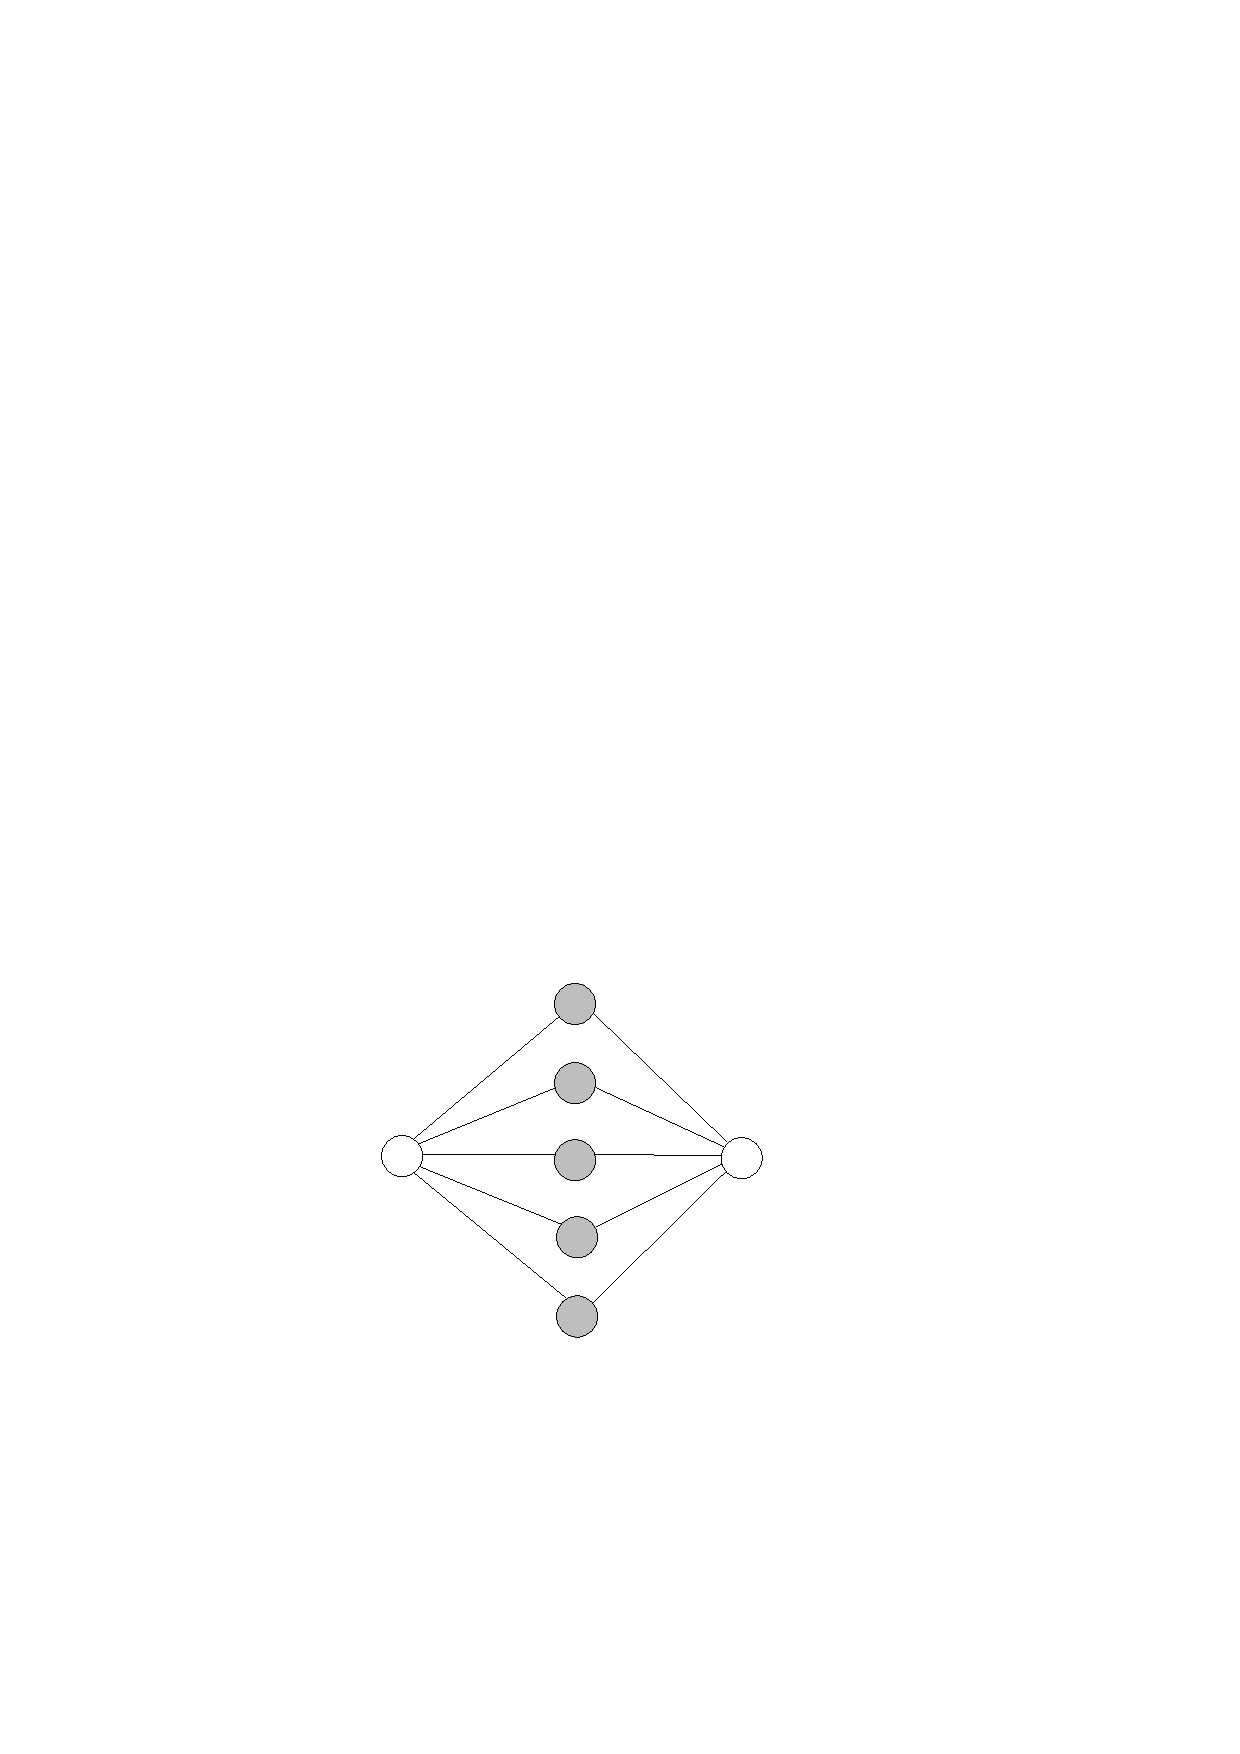
\includegraphics[scale=0.75]{graph.pdf}
\end{answer}
\end{document}
